\documentclass[svgnames,11pt]{beamer}
\input{/home/tof/Documents/Cozy/latex-include/preambule_commun.tex}
\input{/home/tof/Documents/Cozy/latex-include/preambule_beamer.tex}
%\usepackage{pgfpages} \setbeameroption{show notes on second screen=left}
\author[]{Christophe Viroulaud}
\title{Protocole TCP/IP}
\date{\framebox{\textbf{ArchMat 11}}}
%\logo{}
\institute{ Première - NSI }

\begin{document}
\begin{frame}
    \titlepage
\end{frame}
\begin{frame}
    \frametitle{}

    Il y a aujourd'hui plusieurs milliards de machines connectés au réseau \emph{Internet}: ordinateurs, smartphones, télévisions, caméras, frigos\dots
    \begin{framed}
        \centering Comment faire communiquer plusieurs machines ensembles?
    \end{framed}
\end{frame}
\section{Architectures des réseaux}
\begin{frame}
    \frametitle{Architectures des réseaux}

    \begin{center}
        \centering
        \includegraphics[width=9cm]{ressources/local.png}
        \captionof{figure}{\centering Dans un \emph{petit} réseau, les machines sont connectées grâce à un \textbf{switch (connecteur)}.}
        \label{IMG}
    \end{center}

\end{frame}
\begin{frame}
    \frametitle{}
    \begin{aretenir}[]
        Un \textbf{réseau local} est configuré en \textbf{étoile}, autour d'un \textbf{switch}. C'est une solution peu coûteuse et facile à mettre en place. Mais elle n'est pas adaptée aux réseaux trop importants.
    \end{aretenir}


\end{frame}
\begin{frame}
    \frametitle{}

    \begin{center}
        \centering
        \includegraphics[width=9cm]{ressources/maille.png}
        \captionof{figure}{\centering Dans un \emph{gros} réseau, les machines sont connectées grâce à un \textbf{routeur}.}
        \label{IMG}
    \end{center}

\end{frame}
\begin{frame}
    \frametitle{}

    \begin{aretenir}[]
        Un \textbf{réseau maillé} utilise plusieurs \textbf{routeurs} disposés en étoile. C'est une solution plus difficile à mettre en place mais plus robuste: en cas de panne d'un routeur, les messages peuvent emprunter un autre chemin.
    \end{aretenir}

\end{frame}
\begin{frame}
    \frametitle{}

    \begin{center}
        \centering
        \includegraphics[width=9cm]{ressources/reseaux.png}
        \captionof{figure}{\centering \textbf{Internet} est appelé le réseau des réseaux.}
        \label{IMG}
    \end{center}

\end{frame}
\section{Histoire de l'Internet}
\begin{frame}
    \frametitle{Histoire de l'Internet}

    \begin{center}
        \centering
        \includegraphics[width=4cm]{ressources/darpa.png}
        \captionof{figure}{\centering \textbf{1967:} La DARPA (défense américaine) développe le concept de réseau informatique. Elle met rapidement en place le réseau \textbf{ARPANET}}
        \label{IMG}
    \end{center}

\end{frame}
\begin{frame}
    \frametitle{}

    \begin{center}
        \centering
        \includegraphics[width=8cm]{ressources/arpanet.png}
        \captionof{figure}{\centering \textbf{Octobre 1972:} Première démonstration publique du réseau ARPANET}
        \label{IMG}
    \end{center}

\end{frame}
\begin{frame}
    \frametitle{}

    \begin{aretenir}[]
        Le réseau ARPANET est composé de:
        \begin{itemize}
            \item 4 nœuds en 1969 (ouest des États-Unis),
            \item 23 nœuds en 1971,
            \item 111 nœuds en 1974.
        \end{itemize}
        Il relie principalement des universités américaines.
    \end{aretenir}

\end{frame}
\begin{frame}
    \frametitle{}

    \begin{center}
        \centering
        \includegraphics[width=8cm]{ressources/kahncerf.jpg}
        \captionof{figure}{\centering \textbf{1974:} Robert Kahn (droite) et Vinton Cerf (gauche) publient le protocole d'échanges TCP/IP.}
        \label{IMG}
    \end{center}

\end{frame}
\begin{frame}
    \frametitle{}

    \begin{center}
        \centering
        \includegraphics[width=9cm]{ressources/internet.png}
        \captionof{figure}{\centering \textbf{1983:} Le réseau ARPANET est séparé en un réseau militaire et un réseau publique: le terme \textbf{Internet} est adopté.}
        \label{IMG}
    \end{center}

\end{frame}
\section{Le protocole TCP/IP}
\subsection{Présentation}
\begin{frame}
    \frametitle{Le protocole TCP/IP - Présentation}

    \begin{center}
        \begin{tabular}{|c|}
            \hline
            couche application \\
            \hline
            couche transport   \\
            \hline
            couche IP          \\
            \hline
            couche réseau      \\
            \hline
        \end{tabular}
        \captionof{table}{\centering Le protocole est séparé en 4 couches.}
    \end{center}

    \begin{aretenir}[]
        Chaque couche réalise une tâche précise indépendamment des autres.
    \end{aretenir}
\end{frame}
\subsection{Couche réseau}
\begin{frame}
    \frametitle{Couche réseau}

    \begin{aretenir}[]
        La couche réseau transmet l'information \underline{physiquement}:
        \begin{itemize}
            \item par un signal électrique,
            \item par les ondes,
            \item par la lumière.
        \end{itemize}
    \end{aretenir}

\end{frame}
\begin{frame}[fragile]
    \frametitle{}

    \begin{aretenir}[]
        Chaque machine possède une \textbf{adresse MAC (Media Access Control)} unique sur 6 octets; \\exemple: 47:13:b8:31:07:73
    \end{aretenir}
    \begin{center}
        \begin{lstlisting}[language=Bash,basicstyle=\ttfamily\small , xleftmargin=1em, xrightmargin=1em]
ip link
\end{lstlisting}
        \captionof{code}{Récupérer l'adresse MAC de la carte réseau.}
        \label{CODE}
    \end{center}
\end{frame}
\begin{frame}
    \frametitle{}


    \begin{center}
        \centering
        \includegraphics[width=9cm]{ressources/local.png}
        \captionof{figure}{\centering Le commutateur du réseau local connaît les adresses MAC de chaque machine.}
        \label{IMG}
    \end{center}

\end{frame}
\begin{frame}
    \frametitle{}
    \begin{center}
        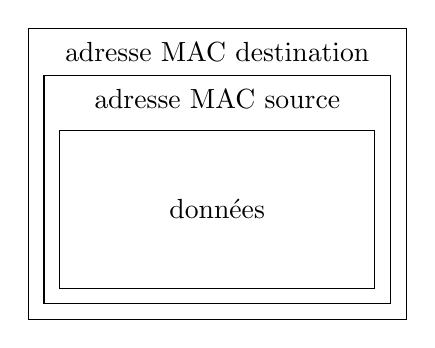
\begin{tikzpicture}
            \draw (-2.2,-1.2) -- (2.2,-1.2) -- (2.2,1.7) -- (-2.2,1.7) -- cycle;
            \node (mac1) at (0,1.4) {adresse MAC source};

            \draw (-2.4,-1.4) -- (2.4,-1.4) -- (2.4,2.3) -- (-2.4,2.3) -- cycle;
            \node (mac2) at (0,2) {adresse MAC destination};

            \node[draw,minimum width=4cm,minimum height=2cm,
                rectangle] (donn) at (0,0) {données};
        \end{tikzpicture}
    \end{center}
    \begin{aretenir}[]
        Les données sont \textbf{encapsulées}: plusieurs couches d'informations sont ajoutées au paquet transmis.
        \\ Le commutateur lit l'adresse de destination dans les premiers octets du paquet.
    \end{aretenir}
\end{frame}
\subsection{Couche IP}
\begin{frame}
    \frametitle{Couche IP}

    \begin{aretenir}[]
        Pour repérer chaque machine sur le réseau Internet, il faut leur fournir une \textbf{adresse IP (Internet Protocol)}.
    \end{aretenir}

\end{frame}
\begin{frame}
    \frametitle{}

    \begin{aretenir}[]
        Une adresse IP (version 4) est composée de \textbf{4 octets}. \\Exemple:
        \begin{center}
            134.87.0.234
        \end{center}
    \end{aretenir}
    \begin{activite}
        \begin{enumerate}
            \item Calculer le nombre d'adresses IPv4 disponibles.
            \item Que peut-on dire du résultat obtenu?
        \end{enumerate}
    \end{activite}

\end{frame}
\begin{frame}
    \frametitle{Correction}

    \begin{itemize}
        \item<1-> $256×256×256×256=256^4=4294967296$ soit plus de 4 milliards d'adresses.
        \item <2-> Ce nombre est insuffisant pour couvrir tous les besoins (ordinateurs, smartphones, objets connectés\dots)
        \item<3-> La nouvelle norme IP (version 6) propose $256^{16}=2^{128}$ adresses (soit environ 3 milliards de milliards de milliards).
    \end{itemize}

\end{frame}
\begin{frame}
    \frametitle{}

    \begin{center}
        \centering
        \includegraphics[width=10cm]{ressources/routage.png}
        \captionof{figure}{\centering Grâce à l'IP de destination, chaque routeur connaît le voisin à qui transmettre le paquet.}
        \label{IMG}
    \end{center}

\end{frame}
\begin{frame}
    \frametitle{}
    \begin{center}
        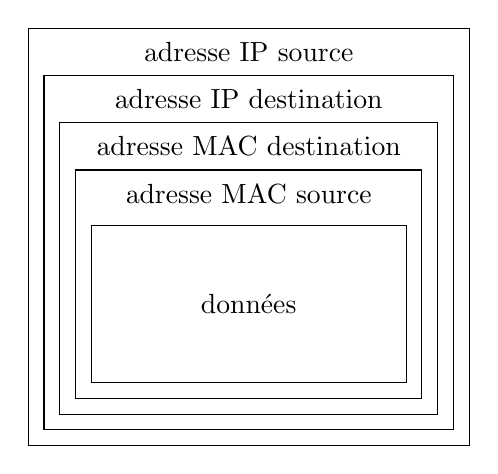
\begin{tikzpicture}
            \draw (-2.2,-1.2) -- (2.2,-1.2) -- (2.2,1.7) -- (-2.2,1.7) -- cycle;
            \node (mac1) at (0,1.4) {adresse MAC source};

            \draw (-2.4,-1.4) -- (2.4,-1.4) -- (2.4,2.3) -- (-2.4,2.3) -- cycle;
            \node (mac2) at (0,2) {adresse MAC destination};

            \draw (-2.6,-1.6) -- (2.6,-1.6) -- (2.6,2.9) -- (-2.6,2.9) -- cycle;
            \node (mac1) at (0,2.6) {adresse IP destination};

            \draw (-2.8,-1.8) -- (2.8,-1.8) -- (2.8,3.5) -- (-2.8,3.5) -- cycle;
            \node (mac1) at (0,3.2) {adresse IP source};

            \node[draw,minimum width=4cm,minimum height=2cm,
                rectangle] (donn) at (0,0) {données};
        \end{tikzpicture}
    \end{center}
    \begin{aretenir}[]
        Les données sont encapsulées. Le routeur lit les adresses IP source et destination. Si elles n'appartiennent pas au même sous-réseau, le paquet est transmis au routeur suivant.
    \end{aretenir}

\end{frame}
\subsection{Couche TCP}
\begin{frame}
    \frametitle{Couche TCP}


    \begin{aretenir}[]
        Le rôle de la couche \textbf{TCP (Transmission Control Protocol)} est de s'assurer de l'intégrité des données transmises et reçues.
    \end{aretenir}

\end{frame}

\begin{frame}
    \frametitle{}

    \begin{activite}
        \underline{Simulation:} Déterminer un protocole qui permet de garantir l'envoi du message intégral.
    \end{activite}

\end{frame}
\begin{frame}
    \frametitle{Correction}

    \begin{itemize}
        \item<1-> Le message est coupé en paquets numérotés.
        \item<2-> Les paquets sont envoyé sur le réseau Internet.
        \item<3-> Le destinataire réceptionne et ordonne les paquets.
        \item<4-> Le destinataire envoie des \textbf{accusés de réception} de chaque paquet reçu.
        \item<5-> Au bout d'un temps déterminé, la source envoie à nouveau un paquet si elle n'a pas reçu l'accusé de réception.
    \end{itemize}
\end{frame}
\begin{frame}
    \frametitle{}

    \begin{aretenir}[Aller plus loin]
        Il existe plusieurs protocoles de transport:
    \begin{itemize}
        \item \textbf{Transmission Control Protocol (TCP):} garantit l'envoi du message intégral grâce à un système d'accusé de réception, mais sans assurance sur la durée.
        \item \textbf{User Datagram Protocol (UDP):} assure une communication plus rapide mais sans assurance sur l'intégrité du message. Il est utilisé, par exemple, pour le streaming.
    \end{itemize}
    \end{aretenir}

\end{frame}
\subsection{Application}
\begin{frame}
    \frametitle{Application}

    \begin{aretenir}[]
    Les données \textbf{décapsulées} par le système d'exploitation, sont utilisées par le logiciel source.
    \end{aretenir}

\end{frame}
\begin{frame}
    \frametitle{}

    \begin{center}
    \centering
    \includegraphics[width=10cm]{ressources/une-minute.jpeg}
    \end{center}

\end{frame}
\begin{frame}
    \frametitle{}

    \begin{center}
    \centering
    \includegraphics[width=10cm]{ressources/uneminute2021.jpeg}
    \end{center}
    
\end{frame}
\end{document}